
%------------------------ Start chapter 3 -------------
\cchapter{روش حل مساله}
\pagebreak

\section{مقدمه}
 
با توجه به کارهای پیشین، مشاهده می‌کنیم که حل مساله با شرایط خاص در جاده و محیط خلوت انجام شده‌است. در این روش‌ها تعداد رنگ‌ها نیز محدود بوده‌است و در پژوهش‌های برتر، رنگ سفید حذف شده‌است، چرا که دشواری مساله را چندین برابر می‌کند. در این رساله، برای اولین بار مساله‌ی تشخیص تابلوهای راهنما و متن آن را در محیط شهری و شلوغ تعریف می‌کنیم. با توجه به این که چنین مجموعه‌ دادگانی به صورت استاندارد وجود ندارد، مجموعه دادگان تهیه و استانداردسازی شده‌است که در فصل بعد به معرفی آن خواهیم پرداخت. سپس در ادامه گام‌های مورد نیاز برای تشخیص تابلو و تشخیص متن فارسی در آن آورده می‌شود \cite{khazaee2016aut}. 


\section{ویژگی‌های تابلوها}
\label{subsec:panelattr}لورم ایپسوم ( به انگلیسی \lr{lorem ipsum} ) متنی بی مفهوم است که تشکیل شده از کلمات معنی دار یا بی معنی کنار هم. کاربر با دیدن متن لورم ایپسوم تصور میکند متنی که در صفحه مشاهده میکند این متن واقعی و مربوط به توضیحات صفحه مورد نظر است واقعی است. حالا سوال اینجاست که این متن « لورم ایپسوم » به چه دردی میخورد و اساسا برای چه منظور و هدفی ساخته شده است؟ پیش از بوجود آمدن لورم ایپسوم ، طراحان وب سایت در پروژه های وب سایت و طراحان کرافیک در پروژه های طراحی کاتولوگ ، بروشور ، پوستر و ... همواره با این مشکل مواجه بودند که صفحات پروژه خود را پیش از آنکه متن اصلی توسط کارفرما ارائه گردد و در صفحه مورد نظر قرار گیرد چگونه پر کنند؟؟ اکثر طراحان با نوشتن یک جمله مانند «این یک متن نمونه است» ویا «توضیحات در این بخش قرار خواهند گرفت» و کپی آن به تعداد زیاد یک یا چند پاراگراف متن میساختند که تمامی متن ها و کلمات ، جملات و پاراگراف ها تکراری بود و از این رو منظره خوبی برای بیننده نداشت و ضمنا به هیچ وجه واقعی به نظر نمیرسید تا بتواند شکل و شمایل تمام شده پروژه را نشان دهد. از این رو متنی ساخته شد که با دو کلمه ( به فارسی : لورم ایپسوم ) آغاز میشد وبا همین نام در بین طراحان وب و گرافیک شناخته و به سرعت محبوب شد. وب سایت های سازنده لورم ایپسوم میتوانند هر تعداد کلمه و پاراگراف که بخواهید به صوورت تکراری یا غیر تکراری برایتان بسازند و تحویلتان بدهند تا از آنها در پروژه هایتان استفاده کنید. ( لورم ایپسوم فارسی) متن های لورم ایپسوم را به زبان فارسی و علاوه بر زبان فارسی به انگلیسی ، عربی ، ترکی استانبولی و ... برایتان میسازد. زبان های دیگر نیز رفته رفته به بانک اطلاعاتی لورم ایسپوم فارسی اضافه خواهند شد.  


\begin{itemize}
\renewcommand{\labelitemii}{$\circ$}

\item مستطیل معمول (\lr{NR})\LTRfootnote{ Normal Rectangle}: 

در این دسته تنها یک قاب در تابلو مشاهده می‌شود. اگر درون تابلو ناحیه‌ی مستطیل شکل با رنگ دیگر ولی بدون قاب جدا کننده وجود داشته باشد، باز هم تابلو از این دسته خواهد بود. یک نمونه در شکل \ref{fig:NR} آورده‌ شده‌است.

\item چند مستطیلی (\lr{MR})\LTRfootnote{ Multiple Rectangles}: 

تابلو در این دسته می‌تواند چندین قاب مستطیلی را در خود جای‌ دهد. این حالت «می‌تواند» در برخی از تابلوهای دارای چند پس‌زمینه رخ می‌دهد. همچنین ممکن است در تابلو با تنها با یک پس‌زمینه، برای تاکید رخ دهد. حالت دیگر، زمانی رخ می‌دهد که چندین تابلوی مستطیل شکل افقی روی هم‌دیگر قرار گرفته باشند. این تابلوها در مجموعه‌دادگان یک تابلو در نظر گرفته شده‌اند و نمونه‌ای از آن‌ را در شکل \ref{fig:MR} مشاهده می‌کنید. 

\item پنج ضلعی (\lr{BP/TP})\LTRfootnote{ Big/Tiny Pentagon}: 

این تابلوها شکل پنج ضلعی دارند که به شکل معمول سر پنج ضلعی به چپ یا راست اشاره می‌کند. این تابلوها به دو شکل بزرگ و کوچک (لاغر) موجود هستند که نمونه‌ی کوچک معمول‌تر است و تفاوت آن با نسخه‌ی بزگ در کشیدگی، پهنای کمتر و در نتیجه بسته‌تر بودن زاویه‌ی علامت پیکان‌مانند آن در سر پنج ضلعی می‌باشد. یک نمونه تابلوی پنج ضلعی بزرگ در شکل \ref{fig:BP} آورده شده‌است. تابلوهای کوچک از این نوع می‌توانند روی هم سوار شوند. 

\item پنج ضلعی با پیکان (\lr{AP})\LTRfootnote{ Arrow Pentagon}: 

این دسته از تابلوها پنج ضلعی با سر اندکی گرد شده هستند و همان‌دسته از تابلوهای نارنجی رنگ سفارشی شهرداری می‌باشند که در این رساله و در این مجموعه دادگان به آن نمی‌پردازیم، چرا که در تصاویر نیز به ندرت دیده می‌شوند. یک نمونه از آن در شکل \ref{fig:AP} آورده شده‌است. 

\end{itemize}
 
 
\begin{figure}[ht]
\centering     %%% not \center
\subfigure[مستطیل معمول \lr{(NR)}]{
\label{fig:NR}
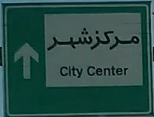
\includegraphics[width=35mm]{NR.png}
}\hspace{-2mm}
\subfigure[چند مستطیلی \lr{(MR)}]{
\label{fig:MR}
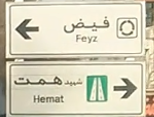
\includegraphics[width=35mm]{MR.png}
}\hspace{-2mm}
\subfigure[پنج ضلعی \lr{(BP/TP)}]{
\label{fig:BP}
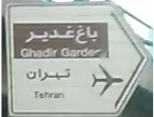
\includegraphics[width=35mm]{BP.png}
}\hspace{-2mm}
\subfigure[پنج ضلعی با پیکان \lr{(AP)}]{
\label{fig:AP}

\includegraphics[width=35mm]{AP.png}
}\hspace{-2mm}
\caption{انواع قاب تابلو}
\end{figure}

 \section{اساس روش پیشنهادی و الگوریتم‌های مورد استفاده}
لورم ایپسوم ( به انگلیسی \lr{lorem ipsum} ) متنی بی مفهوم است که تشکیل شده از کلمات معنی دار یا بی معنی کنار هم. کاربر با دیدن متن لورم ایپسوم تصور میکند متنی که در صفحه مشاهده میکند این متن واقعی و مربوط به توضیحات صفحه مورد نظر است واقعی است. حالا سوال اینجاست که این متن « لورم ایپسوم » به چه دردی میخورد و اساسا برای چه منظور و هدفی ساخته شده است؟ پیش از بوجود آمدن لورم ایپسوم ، طراحان وب سایت در پروژه های وب سایت و طراحان کرافیک در پروژه های طراحی کاتولوگ ، بروشور ، پوستر و ... همواره با این مشکل مواجه بودند که صفحات پروژه خود را پیش از آنکه متن اصلی توسط کارفرما ارائه گردد و در صفحه مورد نظر قرار گیرد چگونه پر کنند؟؟ اکثر طراحان با نوشتن یک جمله مانند «این یک متن نمونه است» ویا «توضیحات در این بخش قرار خواهند گرفت» و کپی آن به تعداد زیاد یک یا چند پاراگراف متن میساختند که تمامی متن ها و کلمات ، جملات و پاراگراف ها تکراری بود و از این رو منظره خوبی برای بیننده نداشت و ضمنا به هیچ وجه واقعی به نظر نمیرسید تا بتواند شکل و شمایل تمام شده پروژه را نشان دهد. از این رو متنی ساخته شد که با دو کلمه ( به فارسی : لورم ایپسوم ) آغاز میشد وبا همین نام در بین طراحان وب و گرافیک شناخته و به سرعت محبوب شد. وب سایت های سازنده لورم ایپسوم میتوانند هر تعداد کلمه و پاراگراف که بخواهید به صوورت تکراری یا غیر تکراری برایتان بسازند و تحویلتان بدهند تا از آنها در پروژه هایتان استفاده کنید. ( لورم ایپسوم فارسی) متن های لورم ایپسوم را به زبان فارسی و علاوه بر زبان فارسی به انگلیسی ، عربی ، ترکی استانبولی و ... برایتان میسازد. زبان های دیگر نیز رفته رفته به بانک اطلاعاتی لورم ایسپوم فارسی اضافه خواهند شد.  

\subsection{رنگ}
لورم ایپسوم ( به انگلیسی \lr{lorem ipsum} ) متنی بی مفهوم است که تشکیل شده از کلمات معنی دار یا بی معنی کنار هم. کاربر با دیدن متن لورم ایپسوم تصور میکند متنی که در صفحه مشاهده میکند این متن واقعی و مربوط به توضیحات صفحه مورد نظر است واقعی است. حالا سوال اینجاست که این متن « لورم ایپسوم » به چه دردی میخورد و اساسا برای چه منظور و هدفی ساخته شده است؟ پیش از بوجود آمدن لورم ایپسوم ، طراحان وب سایت در پروژه های وب سایت و طراحان کرافیک در پروژه های طراحی کاتولوگ ، بروشور ، پوستر و ... همواره با این مشکل مواجه بودند که صفحات پروژه خود را پیش از آنکه متن اصلی توسط کارفرما ارائه گردد و در صفحه مورد نظر قرار گیرد چگونه پر کنند؟؟ اکثر طراحان با نوشتن یک جمله مانند «این یک متن نمونه است» ویا «توضیحات در این بخش قرار خواهند گرفت» و کپی آن به تعداد زیاد یک یا چند پاراگراف متن میساختند که تمامی متن ها و کلمات ، جملات و پاراگراف ها تکراری بود و از این رو منظره خوبی برای بیننده نداشت و ضمنا به هیچ وجه واقعی به نظر نمیرسید تا بتواند شکل و شمایل تمام شده پروژه را نشان دهد. از این رو متنی ساخته شد که با دو کلمه ( به فارسی : لورم ایپسوم ) آغاز میشد وبا همین نام در بین طراحان وب و گرافیک شناخته و به سرعت محبوب شد. وب سایت های سازنده لورم ایپسوم میتوانند هر تعداد کلمه و پاراگراف که بخواهید به صوورت تکراری یا غیر تکراری برایتان بسازند و تحویلتان بدهند تا از آنها در پروژه هایتان استفاده کنید. ( لورم ایپسوم فارسی) متن های لورم ایپسوم را به زبان فارسی و علاوه بر زبان فارسی به انگلیسی ، عربی ، ترکی استانبولی و ... برایتان میسازد. زبان های دیگر نیز رفته رفته به بانک اطلاعاتی لورم ایسپوم فارسی اضافه خواهند شد.  


\begin{figure}[!htb]
\centering     %%% not \center
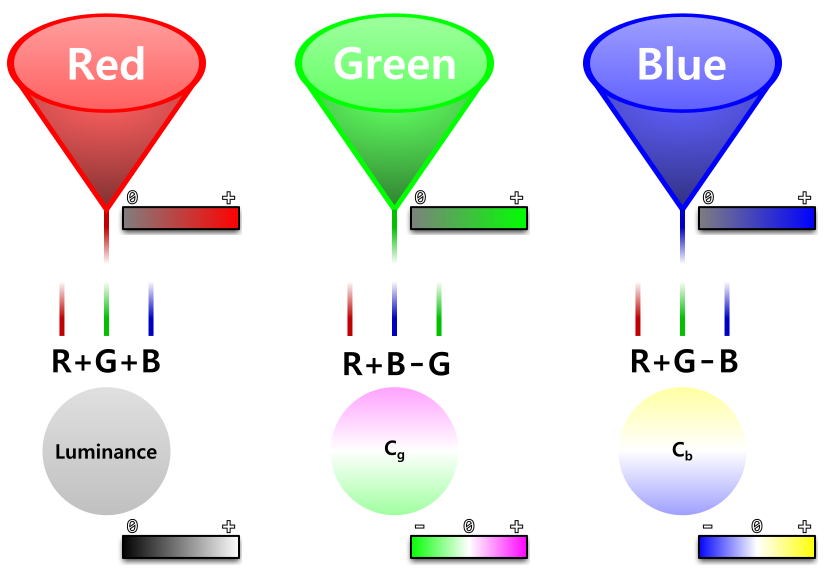
\includegraphics[height=70mm]{oppcolor.png}
\caption[رنگ‌های مخالف]{
پردازش رنگ‌های مخالف در بینایی رنگ \cite{ wiki:hsl}
}
\label{fig:oppcolor}
\end{figure}


\begin{figure}[htb]
\centering     %%% not \center
\subfigure[فیلتر رنگ سفید]{
\label{fig:w}
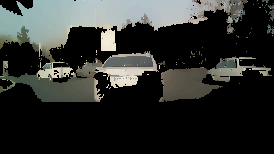
\includegraphics[height=35mm]{w2.png}
}\hspace{-2mm}
\subfigure[فیلتر رنگ سبز]{
\label{fig:g}

\includegraphics[height=35mm]{g2.png}
}
\caption{نمونه فیلترهای رنگ}
\label{fig:color}
\end{figure}


\subsection{روش فلان}

لورم ایپسوم ( به انگلیسی \lr{lorem ipsum} ) متنی بی مفهوم است که تشکیل شده از کلمات معنی دار یا بی معنی کنار هم. کاربر با دیدن متن لورم ایپسوم تصور میکند متنی که در صفحه مشاهده میکند این متن واقعی و مربوط به توضیحات صفحه مورد نظر است واقعی است. حالا سوال اینجاست که این متن « لورم ایپسوم » به چه دردی میخورد و اساسا برای چه منظور و هدفی ساخته شده است؟ پیش از بوجود آمدن لورم ایپسوم ، طراحان وب سایت در پروژه های وب سایت و طراحان کرافیک در پروژه های طراحی کاتولوگ ، بروشور ، پوستر و ... همواره با این مشکل مواجه بودند که صفحات پروژه خود را پیش از آنکه متن اصلی توسط کارفرما ارائه گردد و در صفحه مورد نظر قرار گیرد چگونه پر کنند؟؟ اکثر طراحان با نوشتن یک جمله مانند «این یک متن نمونه است» ویا «توضیحات در این بخش قرار خواهند گرفت» و کپی آن به تعداد زیاد یک یا چند پاراگراف متن میساختند که تمامی متن ها و کلمات ، جملات و پاراگراف ها تکراری بود و از این رو منظره خوبی برای بیننده نداشت و ضمنا به هیچ وجه واقعی به نظر نمیرسید تا بتواند شکل و شمایل تمام شده پروژه را نشان دهد. از این رو متنی ساخته شد که با دو کلمه ( به فارسی : لورم ایپسوم ) آغاز میشد وبا همین نام در بین طراحان وب و گرافیک شناخته و به سرعت محبوب شد. وب سایت های سازنده لورم ایپسوم میتوانند هر تعداد کلمه و پاراگراف که بخواهید به صوورت تکراری یا غیر تکراری برایتان بسازند و تحویلتان بدهند تا از آنها در پروژه هایتان استفاده کنید. ( لورم ایپسوم فارسی) متن های لورم ایپسوم را به زبان فارسی و علاوه بر زبان فارسی به انگلیسی ، عربی ، ترکی استانبولی و ... برایتان میسازد. زبان های دیگر نیز رفته رفته به بانک اطلاعاتی لورم ایسپوم فارسی اضافه خواهند شد.  

\begin{equation}
\begin{aligned}
\mathcal{A}(f) & = \mathfrak{R} \Big( \mathfrak{F} \big[ \mathcal{I}(x) \big] \Big), \\
\mathcal{P}(f) & = \mathfrak{I} \Big( \mathfrak{F} \big[ \mathcal{I}(x) \big] \Big), \\
\mathcal{L}(f) & = \log \Big( \mathcal{A}(f) \Big) , \\
\mathcal{R}(f) & =  \mathcal{L}(f) - h_n(f) \ast  \mathcal{L}(f) ,\\
\mathcal{S}(x) & = g(x) \ast \mathfrak{F}^{-1} \Big[ \exp \big(  \mathcal{R}(f) + \mathcal{P}(f) \big) \Big]^{2} \quad . 
\end{aligned}
\end{equation}
تبدیل فوریه با 
$\mathfrak{F}$
نشان داده شده‌است که بخش حقیقی آن 
$\mathfrak{R}$
، بخش مختلط آن (فاز) 
$\mathfrak{I}$
و
$\mathfrak{F}^{-1}$
تبدیل معکوس فوریه است. همچنین 
 $\mathcal{R}(f)$
  باقی‌مانده‌ی طیفی، 
 $\mathcal{S}(x)$
  نقشه‌ 
 $g(x)$
  فیلتر گاوسی و $h_n$ همانند \eqref{eq:hn} با
   $n=3$
    است. 
\begin{equation}
h_n = {{1} \over {n^2} } 
{
\renewcommand\arraystretch{0.5}
 \begin{pmatrix}
    1 & 1 & \cdots & 1  \\
	1 & 1 & \cdots & 1 \\
	 \vdots & \vdots& \ddots & \vdots  \\
	     1 & 1 & \cdots & 1  \\
  \end{pmatrix}
}
\label{eq:hn}
\end{equation}
	
لورم ایپسوم ( به انگلیسی \lr{lorem ipsum} ) متنی بی مفهوم است که تشکیل شده از کلمات معنی دار یا بی معنی کنار هم. کاربر با دیدن متن لورم ایپسوم تصور میکند متنی که در صفحه مشاهده میکند این متن واقعی و مربوط به توضیحات صفحه مورد نظر است واقعی است. حالا سوال اینجاست که این متن « لورم ایپسوم » به چه دردی میخورد و اساسا برای چه منظور و هدفی ساخته شده است؟ پیش از بوجود آمدن لورم ایپسوم ، طراحان وب سایت در پروژه های وب سایت و طراحان کرافیک در پروژه های طراحی کاتولوگ ، بروشور ، پوستر و ... همواره با این مشکل مواجه بودند که صفحات پروژه خود را پیش از آنکه متن اصلی توسط کارفرما ارائه گردد و در صفحه مورد نظر قرار گیرد چگونه پر کنند؟؟ اکثر طراحان با نوشتن یک جمله مانند «این یک متن نمونه است» ویا «توضیحات در این بخش قرار خواهند گرفت» و کپی آن به تعداد زیاد یک یا چند پاراگراف متن میساختند که تمامی متن ها و کلمات ، جملات و پاراگراف ها تکراری بود و از این رو منظره خوبی برای بیننده نداشت و ضمنا به هیچ وجه واقعی به نظر نمیرسید تا بتواند شکل و شمایل تمام شده پروژه را نشان دهد. از این رو متنی ساخته شد که با دو کلمه ( به فارسی : لورم ایپسوم ) آغاز میشد وبا همین نام در بین طراحان وب و گرافیک شناخته و به سرعت محبوب شد. وب سایت های سازنده لورم ایپسوم میتوانند هر تعداد کلمه و پاراگراف که بخواهید به صوورت تکراری یا غیر تکراری برایتان بسازند و تحویلتان بدهند تا از آنها در پروژه هایتان استفاده کنید. ( لورم ایپسوم فارسی) متن های لورم ایپسوم را به زبان فارسی و علاوه بر زبان فارسی به انگلیسی ، عربی ، ترکی استانبولی و ... برایتان میسازد. زبان های دیگر نیز رفته رفته به بانک اطلاعاتی لورم ایسپوم فارسی اضافه خواهند شد.  

\begin{figure}[p]
\centering     %%% not \center
\subfigure[تصویر اصلی]{
\label{fig:s1}
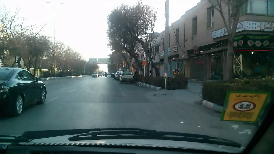
\includegraphics[height=35mm]{s1.png}
}\hspace{-2mm}
\subfigure[نقشه]{
\label{fig:s1o}

\includegraphics[height=35mm]{s1o.png}
}
\subfigure[تصویر اصلی]{
\label{fig:s2}
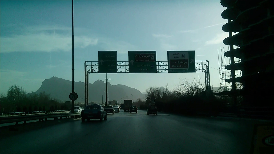
\includegraphics[height=35mm]{s2.png}
}\hspace{-2mm}
\subfigure[نقشه]{
\label{fig:s2o}

\includegraphics[height=35mm]{s2o.png}
}
\subfigure[تصویر اصلی]{
\label{fig:s3}

\includegraphics[height=35mm]{s3.png}
}\hspace{-2mm}
\subfigure[نقشه]{
\label{fig:s3o}

\includegraphics[height=35mm]{s3o.png}
}
\caption[نمونه نقشه‌ها]
{نقشه‌ها در محیط شهری}
\end{figure}
لورم ایپسوم ( به انگلیسی \lr{lorem ipsum} ) متنی بی مفهوم است که تشکیل شده از کلمات معنی دار یا بی معنی کنار هم. کاربر با دیدن متن لورم ایپسوم تصور میکند متنی که در صفحه مشاهده میکند این متن واقعی و مربوط به توضیحات صفحه مورد نظر است واقعی است. حالا سوال اینجاست که این متن « لورم ایپسوم » به چه دردی میخورد و اساسا برای چه منظور و هدفی ساخته شده است؟ پیش از بوجود آمدن لورم ایپسوم ، طراحان وب سایت در پروژه های وب سایت و طراحان کرافیک در پروژه های طراحی کاتولوگ ، بروشور ، پوستر و ... همواره با این مشکل مواجه بودند که صفحات پروژه خود را پیش از آنکه متن اصلی توسط کارفرما ارائه گردد و در صفحه مورد نظر قرار گیرد چگونه پر کنند؟؟ اکثر طراحان با نوشتن یک جمله مانند «این یک متن نمونه است» ویا «توضیحات در این بخش قرار خواهند گرفت» و کپی آن به تعداد زیاد یک یا چند پاراگراف متن میساختند که تمامی متن ها و کلمات ، جملات و پاراگراف ها تکراری بود و از این رو منظره خوبی برای بیننده نداشت و ضمنا به هیچ وجه واقعی به نظر نمیرسید تا بتواند شکل و شمایل تمام شده پروژه را نشان دهد. از این رو متنی ساخته شد که با دو کلمه ( به فارسی : لورم ایپسوم ) آغاز میشد وبا همین نام در بین طراحان وب و گرافیک شناخته و به سرعت محبوب شد. وب سایت های سازنده لورم ایپسوم میتوانند هر تعداد کلمه و پاراگراف که بخواهید به صوورت تکراری یا غیر تکراری برایتان بسازند و تحویلتان بدهند تا از آنها در پروژه هایتان استفاده کنید. ( لورم ایپسوم فارسی) متن های لورم ایپسوم را به زبان فارسی و علاوه بر زبان فارسی به انگلیسی ، عربی ، ترکی استانبولی و ... برایتان میسازد. زبان های دیگر نیز رفته رفته به بانک اطلاعاتی لورم ایسپوم فارسی اضافه خواهند شد.  


سیگنال یک بعدی
 $I : \Omega \rightarrow \mathbb{R}, \Omega = [0 , \infty ) \subset \mathbb{R}$ 
 یک خم $C$ در فضای $\mathbb{R}^2$ می‌سازد. تبدیل ارایه‌شده خم $C$ را از فضایisometric $\mathbb{R}^2$ به فضای $\mathbb{R}$ تبدیل می‌کند به گونه‌ای که فاصله‌ی نقاط اصلی روی خم $C$ با در نظر گرفتن معیاری، حفظ می‌شود. این معیار نرم $l_1$ در نظر گرفته شده‌است، به این معنی که فاصله‌ی نقاط همسایه در تبدیل جدید $(\mathbb{R})$ باید برابر با فاصله‌ی $l_1$ آن‌ها در دامنه‌ی اصلی $(\mathbb{R}^2)$ باشد. تبدیل 
 $ct(x) = t(\hat{x}) = t(x , I(x))$
 را فرض می‌کنیم. لورم ایپسوم ( به انگلیسی \lr{lorem ipsum} ) متنی بی مفهوم است که تشکیل شده از کلمات معنی دار یا بی معنی کنار هم. کاربر با دیدن متن لورم ایپسوم تصور میکند متنی که در صفحه مشاهده میکند این متن واقعی و مربوط به توضیحات صفحه مورد نظر است واقعی است. حالا سوال اینجاست که این متن « لورم ایپسوم » به چه دردی میخورد و اساسا برای چه منظور و هدفی ساخته شده است؟ پیش از بوجود آمدن لورم ایپسوم ، طراحان وب سایت در پروژه های وب سایت و طراحان کرافیک در پروژه های طراحی کاتولوگ ، بروشور ، پوستر و ... همواره با این مشکل مواجه بودند که صفحات پروژه خود را پیش از آنکه متن اصلی توسط کارفرما ارائه گردد و در صفحه مورد نظر قرار گیرد چگونه پر کنند؟؟ اکثر طراحان با نوشتن یک جمله مانند «این یک متن نمونه است» ویا «توضیحات در این بخش قرار خواهند گرفت» و کپی آن به تعداد زیاد یک یا چند پاراگراف متن میساختند که تمامی متن ها و کلمات ، جملات و پاراگراف ها تکراری بود و از این رو منظره خوبی برای بیننده نداشت و ضمنا به هیچ وجه واقعی به نظر نمیرسید تا بتواند شکل و شمایل تمام شده پروژه را نشان دهد. از این رو متنی ساخته شد که با دو کلمه ( به فارسی : لورم ایپسوم ) آغاز میشد وبا همین نام در بین طراحان وب و گرافیک شناخته و به سرعت محبوب شد. وب سایت های سازنده لورم ایپسوم میتوانند هر تعداد کلمه و پاراگراف که بخواهید به صوورت تکراری یا غیر تکراری برایتان بسازند و تحویلتان بدهند تا از آنها در پروژه هایتان استفاده کنید. ( لورم ایپسوم فارسی) متن های لورم ایپسوم را به زبان فارسی و علاوه بر زبان فارسی به انگلیسی ، عربی ، ترکی استانبولی و ... برایتان میسازد. زبان های دیگر نیز رفته رفته به بانک اطلاعاتی لورم ایسپوم فارسی اضافه خواهند شد.  

لورم ایپسوم ( به انگلیسی \lr{lorem ipsum} ) متنی بی مفهوم است که تشکیل شده از کلمات معنی دار یا بی معنی کنار هم. کاربر با دیدن متن لورم ایپسوم تصور میکند متنی که در صفحه مشاهده میکند این متن واقعی و مربوط به توضیحات صفحه مورد نظر است واقعی است. حالا سوال اینجاست که این متن « لورم ایپسوم » به چه دردی میخورد و اساسا برای چه منظور و هدفی ساخته شده است؟ پیش از بوجود آمدن لورم ایپسوم ، طراحان وب سایت در پروژه های وب سایت و طراحان کرافیک در پروژه های طراحی کاتولوگ ، بروشور ، پوستر و ... همواره با این مشکل مواجه بودند که صفحات پروژه خود را پیش از آنکه متن اصلی توسط کارفرما ارائه گردد و در صفحه مورد نظر قرار گیرد چگونه پر کنند؟؟ اکثر طراحان با نوشتن یک جمله مانند «این یک متن نمونه است» ویا «توضیحات در این بخش قرار خواهند گرفت» و کپی آن به تعداد زیاد یک یا چند پاراگراف متن میساختند که تمامی متن ها و کلمات ، جملات و پاراگراف ها تکراری بود و از این رو منظره خوبی برای بیننده نداشت و ضمنا به هیچ وجه واقعی به نظر نمیرسید تا بتواند شکل و شمایل تمام شده پروژه را نشان دهد. از این رو متنی ساخته شد که با دو کلمه ( به فارسی : لورم ایپسوم ) آغاز میشد وبا همین نام در بین طراحان وب و گرافیک شناخته و به سرعت محبوب شد. وب سایت های سازنده لورم ایپسوم میتوانند هر تعداد کلمه و پاراگراف که بخواهید به صوورت تکراری یا غیر تکراری برایتان بسازند و تحویلتان بدهند تا از آنها در پروژه هایتان استفاده کنید. ( لورم ایپسوم فارسی) متن های لورم ایپسوم را به زبان فارسی و علاوه بر زبان فارسی به انگلیسی ، عربی ، ترکی استانبولی و ... برایتان میسازد. زبان های دیگر نیز رفته رفته به بانک اطلاعاتی لورم ایسپوم فارسی اضافه خواهند شد.  


 \begin{equation}
 D(C_1, C_2) = 
 \begin{cases}
    \textit{\lr{true}} & \text{\lr{if} } \ Dif(C_1, C_2) > MInt(C_1, C_2)\\
    false & \text{otherwise}
\end{cases}
 \end{equation}
 
 که در آن کمینه تفاوت داخلی $MInt$ به این صورت تعریف می‌شود‌: 
 \begin{equation}
 MInt(C_1, C_2) = min (Int(C_1) + \tau (C_1), Int(C_2) + \tau (C_2))
 \end{equation}
لورم ایپسوم ( به انگلیسی \lr{lorem ipsum} ) متنی بی مفهوم است که تشکیل شده از کلمات معنی دار یا بی معنی کنار هم. کاربر با دیدن متن لورم ایپسوم تصور میکند متنی که در صفحه مشاهده میکند این متن واقعی و مربوط به توضیحات صفحه مورد نظر است واقعی است. حالا سوال اینجاست که این متن « لورم ایپسوم » به چه دردی میخورد و اساسا برای چه منظور و هدفی ساخته شده است؟ پیش از بوجود آمدن لورم ایپسوم ، طراحان وب سایت در پروژه های وب سایت و طراحان کرافیک در پروژه های طراحی کاتولوگ ، بروشور ، پوستر و ... همواره با این مشکل مواجه بودند که صفحات پروژه خود را پیش از آنکه متن اصلی توسط کارفرما ارائه گردد و در صفحه مورد نظر قرار گیرد چگونه پر کنند؟؟ اکثر طراحان با نوشتن یک جمله مانند «این یک متن نمونه است» ویا «توضیحات در این بخش قرار خواهند گرفت» و کپی آن به تعداد زیاد یک یا چند پاراگراف متن میساختند که تمامی متن ها و کلمات ، جملات و پاراگراف ها تکراری بود و از این رو منظره خوبی برای بیننده نداشت و ضمنا به هیچ وجه واقعی به نظر نمیرسید تا بتواند شکل و شمایل تمام شده پروژه را نشان دهد. از این رو متنی ساخته شد که با دو کلمه ( به فارسی : لورم ایپسوم ) آغاز میشد وبا همین نام در بین طراحان وب و گرافیک شناخته و به سرعت محبوب شد. وب سایت های سازنده لورم ایپسوم میتوانند هر تعداد کلمه و پاراگراف که بخواهید به صوورت تکراری یا غیر تکراری برایتان بسازند و تحویلتان بدهند تا از آنها در پروژه هایتان استفاده کنید. ( لورم ایپسوم فارسی) متن های لورم ایپسوم را به زبان فارسی و علاوه بر زبان فارسی به انگلیسی ، عربی ، ترکی استانبولی و ... برایتان میسازد. زبان های دیگر نیز رفته رفته به بانک اطلاعاتی لورم ایسپوم فارسی اضافه خواهند شد.  

 
 \begin{equation}
 \begin{aligned}
 C_{ab}^* & = \sqrt{a^{*2} + b^{*2}} ,\quad h_{ab} = \arctan \frac{b^{*}}{a^{*}}\\
 \Delta E_{94}^* & = \sqrt{ \left(\frac{\Delta L^*}{k_L S_L}\right)^2 + \left(\frac{\Delta C^*_{ab}}{k_C S_C}\right)^2 + \left(\frac{\Delta H^*_{ab}}{k_H S_H}\right)^2 }, \quad where:\\
 \Delta L^* &= L^*_1 - L^*_2 ,\quad C^*_1 = \sqrt{ {a^*_1}^2 + {b^*_1}^2 } ,\\
 C^*_2 &= \sqrt{ {a^*_2}^2 + {b^*_2}^2 } ,\quad \Delta C^*_{ab} = C^*_1 - C^*_2 \\
 \Delta H^*_{ab} & = \sqrt{ {\Delta E^*_{ab}}^2 - {\Delta L^*}^2 - {\Delta C^*_{ab}}^2 } = \sqrt{ {\Delta a^*}^2 + {\Delta b^*}^2 - {\Delta C^*_{ab}}^2 }\\
 \Delta a^* & = a^*_1 - a^*_2 ,\quad \Delta b^* = b^*_1 - b^*_2, \quad S_L = 1 , \quad S_C = 1+K_1 C^*_1 ,\\
  S_H & = 1+K_2 C^*_1, \quad k_L = 1 , \quad K_1 = 0.045, \quad K_2 = 0.015
  \end{aligned}
 \end{equation}
لورم ایپسوم ( به انگلیسی \lr{lorem ipsum} ) متنی بی مفهوم است که تشکیل شده از کلمات معنی دار یا بی معنی کنار هم. کاربر با دیدن متن لورم ایپسوم تصور میکند متنی که در صفحه مشاهده میکند این متن واقعی و مربوط به توضیحات صفحه مورد نظر است واقعی است. حالا سوال اینجاست که این متن « لورم ایپسوم » به چه دردی میخورد و اساسا برای چه منظور و هدفی ساخته شده است؟ پیش از بوجود آمدن لورم ایپسوم ، طراحان وب سایت در پروژه های وب سایت و طراحان کرافیک در پروژه های طراحی کاتولوگ ، بروشور ، پوستر و ... همواره با این مشکل مواجه بودند که صفحات پروژه خود را پیش از آنکه متن اصلی توسط کارفرما ارائه گردد و در صفحه مورد نظر قرار گیرد چگونه پر کنند؟؟ اکثر طراحان با نوشتن یک جمله مانند «این یک متن نمونه است» ویا «توضیحات در این بخش قرار خواهند گرفت» و کپی آن به تعداد زیاد یک یا چند پاراگراف متن میساختند که تمامی متن ها و کلمات ، جملات و پاراگراف ها تکراری بود و از این رو منظره خوبی برای بیننده نداشت و ضمنا به هیچ وجه واقعی به نظر نمیرسید تا بتواند شکل و شمایل تمام شده پروژه را نشان دهد. از این رو متنی ساخته شد که با دو کلمه ( به فارسی : لورم ایپسوم ) آغاز میشد وبا همین نام در بین طراحان وب و گرافیک شناخته و به سرعت محبوب شد. وب سایت های سازنده لورم ایپسوم میتوانند هر تعداد کلمه و پاراگراف که بخواهید به صوورت تکراری یا غیر تکراری برایتان بسازند و تحویلتان بدهند تا از آنها در پروژه هایتان استفاده کنید. ( لورم ایپسوم فارسی) متن های لورم ایپسوم را به زبان فارسی و علاوه بر زبان فارسی به انگلیسی ، عربی ، ترکی استانبولی و ... برایتان میسازد. زبان های دیگر نیز رفته رفته به بانک اطلاعاتی لورم ایسپوم فارسی اضافه خواهند شد.  
 
%------------------------ End chapter 3 -------------
